%Vienna.tex
%
%  Talk for University of Vienna Colloquium: 
%   Bounds for real solutions to structured polynomial systesm
%
% The basic document style is 'foils' from the FoilTeX package
\documentclass[17pt,landscape]{Narrow}
%
%   Narrow is the corect width for most projections
%
% These are my macros for creating slides
\usepackage{mdwslides}

% Basic things that we need are below
\usepackage[english]{babel}
\usepackage{hyperref}
\hypersetup{
  pdfmenubar=true,
  pdftoolbar=true,
  pdfpagemode={None}
}
\usepackage{pause}
\usepackage{graphicx,amssymb,amsmath}
\usepackage{colordvi}

\newcommand{\DeCo}{\RoyalBlue}

\newcommand{\ba}{\mathbf{a}}
\newcommand{\bb}{\mathbf{b}}

\newcommand{\conv}{\mbox{\sf conv}}
\newcommand{\vol}{\mbox{\sf vol}}

\renewcommand{\P}{{\mathbb P}}
\newcommand{\C}{{\mathbb C}}
\newcommand{\N}{{\mathbb N}}
\newcommand{\R}{{\mathbb R}}
\newcommand{\Z}{{\mathbb Z}}
\newcommand{\calA}{{\mathcal A}}


%%%%%%%%%%%%%%%%%%%%%%%%%%%%%%%%%%%%%%%%%%%%%%%%%%%%%%%%%%%%%%%%%%%%%%%%%%%%
\textheight=125mm     \textwidth=180mm
\topmargin=-27mm
\oddsidemargin=-20mm   \evensidemargin=-20mm
%%%%%%%%%%%%%%%%%%%%%%%%%%%%%%%%%%%%%%%%%%%%%%%%%%%%%%%%%%%%%%%%%%%%%%%%%%%%

% Set headers
\MyLogo{\Maroon{Frank Sottile, Texas A\&M University}}
\rightfooter{\quad\textsf{\thepage}}

\begin{document}
\sf

\slide{}
\LogoOff
\thispagestyle{empty}

\begin{center}\rule{0pt}{30pt}
\Blue{{\LARGE Bounds for real solutions to structured polynomial systems}}\rule{0pt}{25pt}\\
\large Colloquium, Department of Mathematics\rule{0pt}{30pt}\\
University of Vienna\\
15 October 2008\vspace{-30pt}

%\vskip 1ex

\hfill\makebox[7cm][l]{\hspace{-145pt}{\includegraphics[width=12cm]{FRSC.eps}}}\vspace{-115pt}

\noindent\hspace{-10pt}

\includegraphics[width=3cm]{tamuseal.eps}
\begin{minipage}[b]{8cm}
Frank Sottile\\
{\small\tt sottile@math.tamu.edu}
\end{minipage}\rule{100pt}{0pt}


\end{center}

%%%%%%%%%%%%%%%%%%%%%%%%%%%%%%%%%%%%%%%%%%%%%%%%%%%%%%%%%%%%%%

\setcounter{page}{0}
\begin{flushleft}
%%%%%%%%%%%%%%%%%%%%%%%%%%%%%%%%%%%%%%%%%%%%%%%%%%%%%%%%%%%%%%
\slide{}
\LogoOn
\begin{center}
\RawSienna{{\LARGE Bounds for real solutions}}
\end{center}

Given a system of polynomials\vspace{-8pt}
\[
   f_1(x_2,\dotsc,x_n)\ =\  \dotsb\ =\ f_N(x_1,\dotsc,x_n)\ =\ 0\,,\vspace{-8pt}
\]
with \DeCo{$d$} nondegenerate complex solutions, what can we say about its number, 
\DeCo{$r$}, of real solutions, (besides the trivial\vspace{-8pt}
\[
    d\ \geq\ r\ \geq\ d\mod 2 \in\{0,1\}\ ?\,)\vspace{-8pt}
\]
While the answer in general is {\sl nothing}, when the equations have special structure
coming from geometry, we can often say a great deal about $r$,
or the positive solutions, \DeCo{$r_+$}.\vspace{-8pt}

\begin{itemize}
 \item[$\bullet$] Sometimes, there is a smaller, sharp upper bound than $d$
 \item[$\bullet$] Often, there is a lower bound larger than $d\mod 2$
 \item[$\bullet$] In some cases the lower bound is $d$.\vspace{-8pt}
\end{itemize}


%%%%%%%%%%%%%%%%%%%%%%%%%%%%%%%%%%%%%%%%%%%%%%%%%%%%%%%%%%%%%%
%%%%%%%%%%%%%%%%%%%%%%%%%%%%%%%%%%%%%%%%%%%%%%%%%%%%%%%%%%%%%%
\slide{}
\LogoOn
\begin{center}
\RawSienna{{\LARGE Complex bounds for sparse systems}}
\end{center}

\noindent
An integer vector $\alpha=(a_1,\dotsc,a_n)\in\Z^n$ \newline
corresponds to a (Laurent) monomial, $\DeCo{x^\alpha}:= x_1^{a_1} \dotsc x_n^{a_n}$.

A polynomial with \DeCo{support} $\calA\subset\Z^n$ is\vspace{-8pt}
\[
   f\ =\ \sum_{\alpha\in \calA} c_\alpha x^\alpha
   \qquad c_\alpha\in\R (\ \mbox{or}\ \in\C)\,.\vspace{-8pt}
\]

\noindent\Brown{Kushnirenko's Theorem.}
{\sl 
 A general system of polynomials\vspace{-8pt}
\[
   f_1(x_1,\dotsc,x_n)\ =\ \dotsb\ =\ f_n(x_1,\dotsc,x_n)\ =\ 0\vspace{-8pt}
\]
with support $f_i=\calA$ has 
$d=n!\vol(\conv(\calA))$ solutions.
}

\noindent\Brown{Bernstein's Theorem.}
{\sl 
If the polynomials have different supports,  $\calA_1,\dotsc,\calA_n$,
then $d=$ mixed volume of $\conv(\calA_i),\ i=1,\dotsc,n$.
}


%%%%%%%%%%%%%%%%%%%%%%%%%%%%%%%%%%%%%%%%%%%%%%%%%%%%%%%%%%%%%%
%%%%%%%%%%%%%%%%%%%%%%%%%%%%%%%%%%%%%%%%%%%%%%%%%%%%%%%%%%%%%%
\slide{}
\LogoOn
\begin{center}
\RawSienna{{\LARGE Upper bounds}}%: from Descartes to Khovanski}}
\end{center}

By Descartes' rule of signs ({\sl c}. 1637),\vspace{-8pt}
\[
  c_0x^{a_0} \,+\,c_1x^{a_1}\,+\,\dotsb\,+\,c_nx^{a_n}\ =\ 0\,\vspace{-8pt}
\]
has $r_+\leq n$ ( $\leq n$ positive solutions).

Khovanskii ({\sl c}. 1980) gave a multivariate generalization.\vspace{-5pt}

\noindent\Brown{Theorem.}
{\sl
% The number of positive solutions to a system of polynomials\vspace{-8pt}
 A system of polynomial equations\vspace{-8pt}
\[
   f_1(x_1,\dotsc,x_n)\ =\ \dotsb\ =\ f_n(x_1,\dotsc,x_n)\ =\ 0\vspace{-8pt}
\]
% with $1+l+n$ monomials (e.g. $|\calA|=1+l+n$) is less than\vspace{-8pt}
 with $1+l+n$ monomials (e.g. $|\calA|=1+l+n$) has\vspace{-8pt}
\[
   r_+\ <\ 
   2^{\binom{l+n}{2}}(n+1)^{l+n}\,.\vspace{-25pt}
\]
}

\noindent
$\Rightarrow$ $r_+$ has a completely different character than $d$.


%\vspace{-8pt}

%%%%%%%%%%%%%%%%%%%%%%%%%%%%%%%%%%%%%%%%%%%%%%%%%%%%%%%%%%%%%%
%%%%%%%%%%%%%%%%%%%%%%%%%%%%%%%%%%%%%%%%%%%%%%%%%%%%%%%%%%%%%%
\slide{}
\LogoOn
\begin{center}
\RawSienna{{\LARGE New upper bounds}}
\end{center}

Khovanski more generally gave a topological method to bound solutions to
systems of equations.
Significant improvements to his bound have recently been found that take advantage of some (simple)
geometry and combinatorics available for systems of polynomials.\vspace{-5pt}

\noindent
Given a system with support $\calA$ where $|\calA|=1{+}l{+}n$,\vspace{-8pt}
\[
   f_1(x_1,\dotsc,x_n)\ =\ \dotsb\ =\ f_n(x_1,\dotsc,x_n)\ =\ 0\,.\vspace{-18pt}
\]

\noindent\Brown{Theorem (Bihan-S.).}
{\sl We have \vspace{-8pt}
\[ 
r_+ \ <\   \sum_{j=1}^l 2^{\binom{l-j}{2}}n^{l-j}\tbinom{n{+}l{+}1}{j}
  \ <\  \tfrac{e^2+3}{4}2^{\binom{l}{2}}n^l\,.\vspace{-18pt}
\]
}

\noindent\Brown{Theorem (Bates-Bihan-S.).}
{\sl When $\calA$ is \DeCo{primitive}, \ $\DeCo{r} < \frac{e^{\DeCo{4}}+3}{4}2^{\binom{l}{2}}n^l$. }


\noindent\Brown{Theorem (Bihan-Rojas-S.).}
{\sl These are sharp for $l$ fixed and $n\gg 0$.}

%\vspace{-8pt}
%\vspace{-8pt}
%%%%%%%%%%%%%%%%%%%%%%%%%%%%%%%%%%%%%%%%%%%%%%%%%%%%%%%%%%%%%%
%%%%%%%%%%%%%%%%%%%%%%%%%%%%%%%%%%%%%%%%%%%%%%%%%%%%%%%%%%%%%%
\slide{}
\LogoOn
\begin{center}
\RawSienna{{\LARGE Three challenges}}
\end{center}

The fewnomial bounds\vspace{-8pt}
\[
   2^{\binom{l+n}{2}}(n+1)^{l+n}\qquad\mbox{and}\qquad
\tfrac{e^2+3}{4}2^{\binom{l}{2}}n^l\vspace{-8pt}
\]
are both exponential in $l^2$.\newline
\noindent\Brown{Challenge 1.}  Find a bound with lower order in $l$.

It is easy to construct systems with $O(l^n)$ real solutions.\newline
\noindent\Brown{Challenge 2.} Construct systems with more real soutions.

These results are for systems of polynomials with the same supports.\newline
\noindent\Brown{Challenge 3.} Give bounds for polynomials with different supports.


%\vspace{-8pt}
%%%%%%%%%%%%%%%%%%%%%%%%%%%%%%%%%%%%%%%%%%%%%%%%%%%%%%%%%%%%%%
%%%%%%%%%%%%%%%%%%%%%%%%%%%%%%%%%%%%%%%%%%%%%%%%%%%%%%%%%%%%%%
\slide{}
\LogoOn
\begin{center}
\RawSienna{{\LARGE Lower bounds}}
\end{center}

Many geometric problems enjoy a non-trivial lower bound on their number of real solutions,
which is an existence proof for real solutions.

The most spectacular such bound concerns the number \DeCo{$N_d$} of plane rational curves
of degree $d$ interpolating $3d-1$ points in $\C\P^2$.
$N_1=1$, as two points determine a line.
Around 1990 Kontsevich gave the elegant recursion that starts with $N_1=1$,
\[
  N_d\ =\   \sum_{a+b=d} N_a N_b \left( a^2b^2\tbinom{3d-4}{3a-2} - 
           a^3b\tbinom{3d-4}{3a-1}\right)\ .
\]

If the points lie in $\R\P^2$, how many of the curves $C$ can be real?

%\vspace{-8pt}
%%%%%%%%%%%%%%%%%%%%%%%%%%%%%%%%%%%%%%%%%%%%%%%%%%%%%%%%%%%%%%
%%%%%%%%%%%%%%%%%%%%%%%%%%%%%%%%%%%%%%%%%%%%%%%%%%%%%%%%%%%%%%
\slide{}
\setcounter{page}{7}

\LogoOn
\begin{center}
\RawSienna{{\LARGE Welchsinger invariant}}
\end{center}

Real rational curves have 3 types of singularities:
\[
 \begin{picture}(450,80)
  \put(0,15){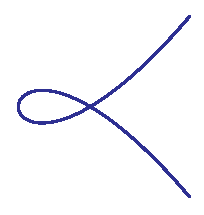
\includegraphics[height=75pt]{renodes.eps}}
  \put(22,0){node}
  \put(130,15){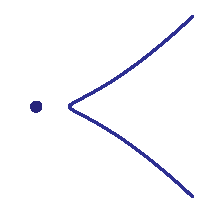
\includegraphics[height=75pt]{conodes.eps}}
  \put(130,0){solitary point}

  \put(270,0){\White{complex conjugate nodes}}
 \end{picture}
\]

\noindent\White{Welschinger's Theorem.}
 \White{The sum}\vspace{-8pt}
\[
    \White{\sum (-1)^{\mbox{\# solitary points in $C$}}\,,}\vspace{-8pt}
\]
\White{{\sl over all real $C$ interpolating $3d-1$ points in $\R\P^2$, is independent of 
the choice of points.
}}

\White{This number is the {Welschinger invariant}, {$W_d$}.\newline 
$|W_d|$ is a lower bound for the
  number of interpolating real curves.}

%\vspace{-8pt}
%%%%%%%%%%%%%%%%%%%%%%%%%%%%%%%%%%%%%%%%%%%%%%%%%%%%%%%%%%%%%%
%%%%%%%%%%%%%%%%%%%%%%%%%%%%%%%%%%%%%%%%%%%%%%%%%%%%%%%%%%%%%%
\slide{}
\setcounter{page}{7}

\LogoOn
\begin{center}
\RawSienna{{\LARGE Welchsinger invariant}}
\end{center}

Real rational curves have 3 types of singularities:
\[
 \begin{picture}(450,80)
  \put(0,15){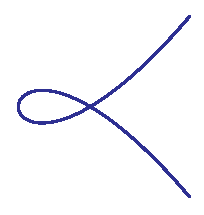
\includegraphics[height=75pt]{renodes.eps}}
  \put(22,0){node}
  \put(130,15){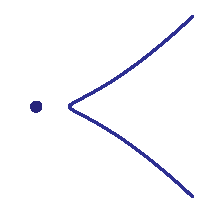
\includegraphics[height=75pt]{conodes.eps}}
  \put(130,0){solitary point}

  \put(270,0){complex conjugate nodes}
 \end{picture}
\]

\noindent\Brown{Welschinger's Theorem.}
{\sl  The sum\vspace{-8pt}
\[
    \sum (-1)^{\mbox{\# solitary points in $C$}}\,,\vspace{-8pt}
\]
over all real $C$ interpolating $3d-1$ points in $\R\P^2$, is independent of 
the choice of points.
}

This number is the \DeCo{Welschinger invariant}, \DeCo{$W_d$}.\newline 
$|W_d|$ is a lower bound for the number of interpolating real curves.

%\vspace{-8pt}
%%%%%%%%%%%%%%%%%%%%%%%%%%%%%%%%%%%%%%%%%%%%%%%%%%%%%%%%%%%%%%
%%%%%%%%%%%%%%%%%%%%%%%%%%%%%%%%%%%%%%%%%%%%%%%%%%%%%%%%%%%%%%
\slide{}
\LogoOn
\begin{center}
\RawSienna{{\LARGE Tropical interpolation}}
\end{center}

Mikhalkin gave different formulae for $N_d$ and $W_d$ via counting 
tropical curves with multiplicities.\vspace{-8pt} 
\[
  \begin{matrix}
   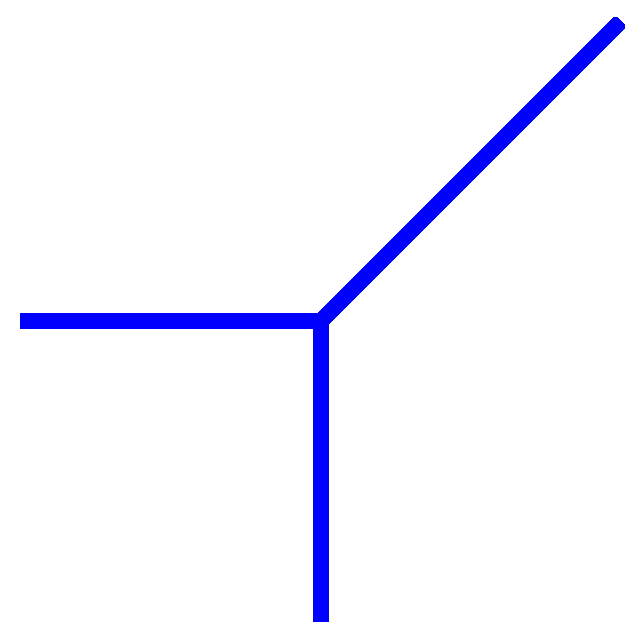
\includegraphics[width=55pt]{Tline.eps}&\ &
   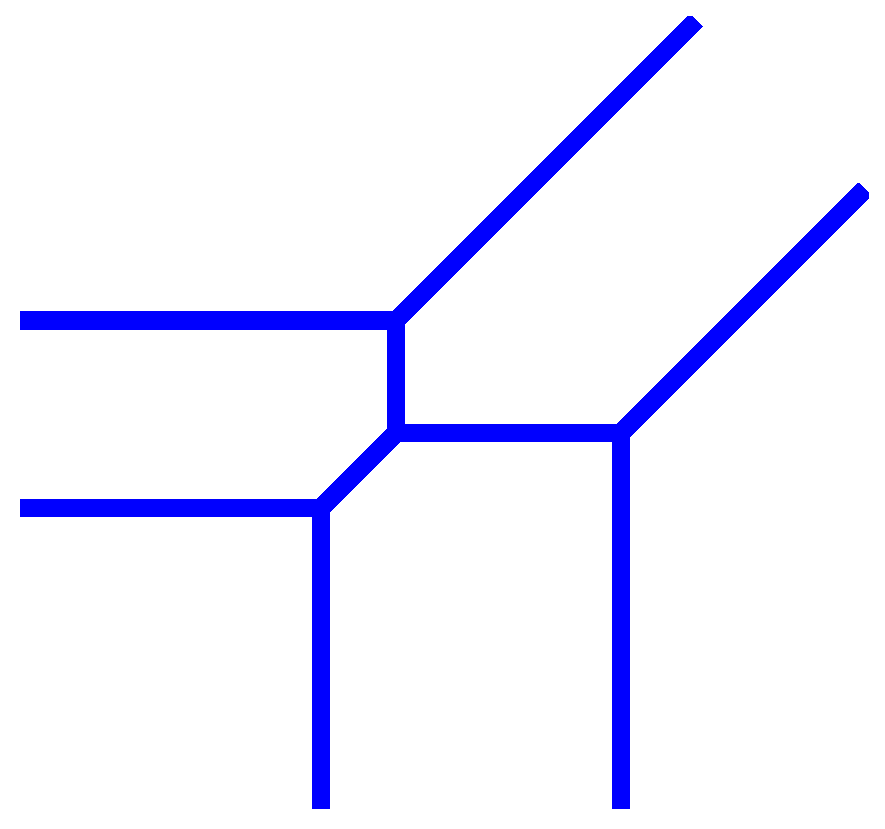
\includegraphics[width=65pt]{TConic.eps}&\ &
   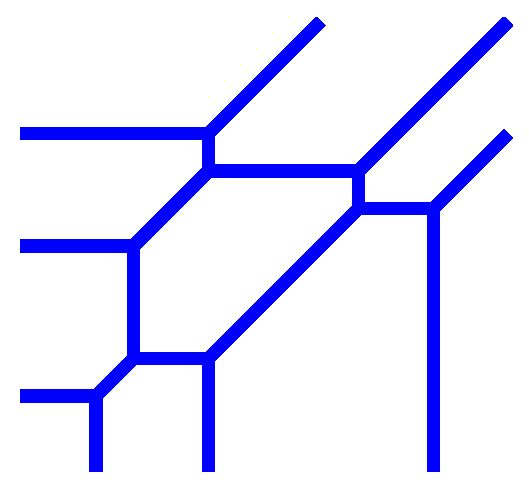
\includegraphics[width=65pt]{TCubic.eps}&\ & 
   \begin{picture}(65,65)
      \put(0,0){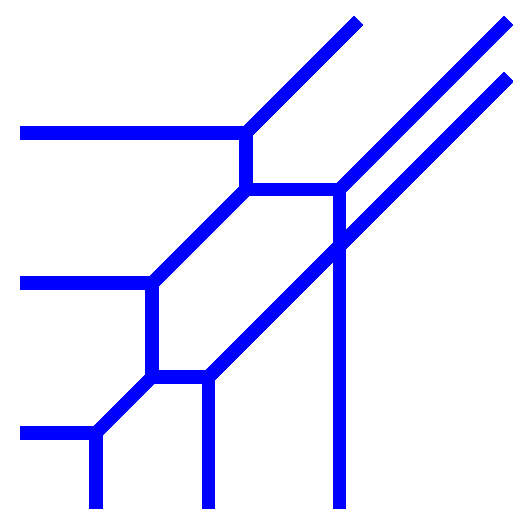
\includegraphics[width=65pt]{TNode.eps}}
      \put(54,23.5){\vector(-1,1){10}}   
      \put(50,16){node}
    \end{picture}\\
  \text{line}&&\text{conic}&&\text{cubic}&&\text{rational cubic}
  \end{matrix}\vspace{-8pt}
\]

Using this, Itenberg, Kharlamov, and Shustin obtained the following:\vspace{-8pt}
\begin{itemize}
 \item[$\bullet$]  $W_d\geq \tfrac{d!}{3}\ (>0)$,
 \item[$\bullet$]  $\lim_{d\to\infty} \log(N_d)/\log(W_d)\ =\ 1$\,,
 \item[$\bullet$]  A recursion for $W_d$.
\end{itemize}

Recently, Solomon showed $W_d$ is the degree of a map.
%\vspace{-8pt}
%\vspace{-8pt}
%%%%%%%%%%%%%%%%%%%%%%%%%%%%%%%%%%%%%%%%%%%%%%%%%%%%%%%%%%%%%%
%%%%%%%%%%%%%%%%%%%%%%%%%%%%%%%%%%%%%%%%%%%%%%%%%%%%%%%%%%%%%%
\slide{}
\LogoOn
\begin{center}
\RawSienna{{\LARGE Wronski map}}
\end{center}

The  Wronskian, $\mbox{Wr}:=\det|(\frac{d}{d t})^i f_j(t)|$ of
univariate polynomials $f_1(t),\dotsc,f_k(t)$ of degree $d$, has degree $k(d{+}1{-}k)$.
Up to a scalar, it depends only on the linear span of the $f_j$, and 
defines a map\vspace{-8pt}
\[
   \DeCo{\mbox{Wr}}\ \colon\ \mbox{Grass}(k,d{+}1) \ \longrightarrow\ \C\P^{k(d+1-k)}\vspace{-8pt}
\]
of degree the number of Young tableaux of shape $k\times(d{+}1{-}k)$.

A Young tableau $T$ is a linear extension of the product of chains of lengths $k$
and $d{+}1{-}k$ and therefore has a sign $\sigma(T)\in{\pm1}$.


\Brown{Theorem (Eremenko-Gabrielov).} 
If $W(x)\in\R\P^{k(d+1-k)}$, then \vspace{-8pt}
\[
   \# \mbox{Wr}_\R^{-1}(W(x))\ \geq\  |\sum_T \sigma(T)|\,.\vspace{-18pt}
\]

\Brown{Proof.} The degree of real Wronski map equals RHS \newline ($=$ sign-imbalance of product of
chains of lengths $k$ and $d{+}1{-}k$). 
%\vspace{-8pt}
%%%%%%%%%%%%%%%%%%%%%%%%%%%%%%%%%%%%%%%%%%%%%%%%%%%%%%%%%%%%%%
%%%%%%%%%%%%%%%%%%%%%%%%%%%%%%%%%%%%%%%%%%%%%%%%%%%%%%%%%%%%%%
\slide{}
\LogoOn
\begin{center}
\RawSienna{{\LARGE Lower bounds for sparse systems}}
\end{center}

Soprunova and I began to develop a theory of lower bounds for systems of polynomials with
support $\calA$.  
Its first step was to formulate a polynomial system as the fiber of a map 
$\pi\colon X_\calA\to\R\P^n$ from a real toric variety $X_\calA$.\vspace{-4pt}

\begin{itemize}
 \item[$\to$] Give conditions on $\mbox{conv}(\calA)$ when $\pi$ has a degree.
 \item[$\to$] Give a method to compute this degree in a special case (foldable triangulations).
 \item[$\to$] Use this method to compute degree for polynomial systems from a poset $P$,
              where the degree is the sign-imbalance of $P$.
 \item[$\to$] Use this and SAGBI degenerations to give new proof of Eremenko-Gabrielov
              theorem.\vspace{-4pt} 
\end{itemize}

Joswig and Witte found many more examples coming from foldable triangulations.



%\vspace{-8pt}
%%%%%%%%%%%%%%%%%%%%%%%%%%%%%%%%%%%%%%%%%%%%%%%%%%%%%%%%%%%%%%
%%%%%%%%%%%%%%%%%%%%%%%%%%%%%%%%%%%%%%%%%%%%%%%%%%%%%%%%%%%%%%
\slide{}
\LogoOn
\begin{center}
\RawSienna{{\LARGE When lower bound = upper bound}}
\end{center}

The Wronski map\vspace{-8pt}
\[
   \mbox{Wr}\ \colon\ \mbox{Grass}(k,d{+}1) \ \longrightarrow\ \C\P^{k(d+1-k)}\vspace{-8pt}
\]
takes a $k$-plane of univariate polynomials to its Wronski determinant.


\Brown{Theorem (Mukhin-Tarasov-Varchenko).}
{\sl 
 If a polynomial $\Phi\in\R\P^{k(d+1-k)}$ has only real roots, then
 every $k$-plane in $\mbox{\sf Wr}^{-1}(\Phi)$ is real.
}

Earlier, Eremenko and Gabrielov proved this when $k=2$.

\Brown{Theorem.}
{\sl 
  A rational function with real critical points is real.
}

These results concern the Shapiro conjecture in Schubert calculus.

\Magenta{{\sf Go to animation}}

%\vspace{-8pt}
%%%%%%%%%%%%%%%%%%%%%%%%%%%%%%%%%%%%%%%%%%%%%%%%%%%%%%%%%%%%%%
%%%%%%%%%%%%%%%%%%%%%%%%%%%%%%%%%%%%%%%%%%%%%%%%%%%%%%%%%%%%%%
\slide{}
\LogoOn
\begin{center}
\RawSienna{{\LARGE Schubert calculus}}
\end{center}

A partition \DeCo{$\lambda$} and a flag \DeCo{$F_\bullet$} in $\C^{d+1}$
together determine a \newline\DeCo{Schubert variety},
$\DeCo{X_\lambda F_\bullet}\subset\mbox{Grass}(k,d{+}1)$.

$\DeCo{|\lambda|}\ :=$ codimension of $X_\lambda F_\bullet$.

Given partitions $\lambda_1,\dotsc,\lambda_m$ with 
$\sum|\lambda_i|\ =\mbox{\sf dim}(\mbox{Grass})$ and\newline
general flags $F_\bullet^1,\dotsc,F_\bullet^m$,

\Brown{Kleiman's Theorem} implies that\vspace{-8pt}
\[
   \bigcap_{i=1}^m X_{\lambda_i}F_\bullet^i\vspace{-8pt}
\]
 is transverse and consists of
$d=d(\lambda_1,\dotsc,\lambda_m)$ $k$-planes in $\C^{d+1}$.




%\vspace{-8pt}
%%%%%%%%%%%%%%%%%%%%%%%%%%%%%%%%%%%%%%%%%%%%%%%%%%%%%%%%%%%%%%
%%%%%%%%%%%%%%%%%%%%%%%%%%%%%%%%%%%%%%%%%%%%%%%%%%%%%%%%%%%%%%
\slide{}
\LogoOn
\begin{center}
\RawSienna{{\LARGE Shapiro Conjecture}}
\end{center}


For $z\in\C$, the space $\C_d[t]$ of polynomials
of degree $\leq d$ has a flag $F_\bullet(z)$ 
whose $i$-space consists of polynomials which vanish to order
at least $d{+}1{-}i$ at $z$.

\Brown{Shapiros's Conjecture (Mukhin-Tarasov-Varchenko Theorem).}\newline
{\sl 
   If $z_1,\dotsc,z_m$ are distinct and \DeCo{real}, then\vspace{-8pt}
\[
   \bigcap_{i=1}^m X_{\lambda_i}F_\bullet(z_i)\vspace{-8pt}
\]
 is transverse and consists of $d(\lambda_1,\dotsc,\lambda_m)$ \DeCo{real} $k$-planes. 
}

\begin{itemize}
\item[\Red{$\to$}] One proof (there are three) gives deep connection to representation theory.

\item[\Red{$\leadsto$}] Interesting combinatorial question concerning monodromy and Young tableaux.
\end{itemize}
%\vspace{-8pt}
%%%%%%%%%%%%%%%%%%%%%%%%%%%%%%%%%%%%%%%%%%%%%%%%%%%%%%%%%%%%%%
%%%%%%%%%%%%%%%%%%%%%%%%%%%%%%%%%%%%%%%%%%%%%%%%%%%%%%%%%%%%%%
\slide{}
\LogoOn
\begin{center}
\RawSienna{{\LARGE Monodromy}}
\end{center}

The fibration\vspace{-8pt}
\[
    \bigcap_{i=1}^m X_{\lambda_i} F_\bullet(z_i)\  \longrightarrow\ 
      (z_1,\dotsc,z_m)\ \in\ (\R\P^1)\setminus\Delta\vspace{-8pt}
\]
has base with components necklaces (points $z_i$ of $\R\P^1$ labeled by
partition $\lambda_i$) and each component is homeomorphic to $\R\P^1$.

Fibers naturally labeled by an interesting set of Young tableaux.

\Brown{Question.}  What is the monodromy?

Purbhoo has shown it is essentially Sch\"utzenberger evacuation and {\sl jeu-de-taquin}.

%%%%%%%%%%%%%%%%%%%%%%%%%%%%%%%%%%%%%%%%%%%%%%%%%%%%%%%%%%%%%%
\end{flushleft}
\end{document}

%%%%%%%%%%%%%%%%%%%%%%%%%%%%%%%%%%%%%%%%%%%%%%%%%%%%%%%%%%%%%%
\slide{}
\LogoOn
\begin{center}
\RawSienna{{\LARGE Link to representation theory}}
\end{center}

\DeCo{${\mathcal O}$} $:=$ coordinate ring of big cell of Grass.

${\mathcal O}\twoheadrightarrow \cap X_{\lambda^i}F_\bullet(z_i)$ is indexed by
$z_1,\dotsc,z_m$.

Evaluation module \DeCo{$V_\lambda(z)$} is an irreducible representation of ${\mathfrak sl}_k[t]$.

$\DeCo{B}

%\vspace{-8pt}
%%%%%%%%%%%%%%%%%%%%%%%%%%%%%%%%%%%%%%%%%%%%%%%%%%%%%%%%%%%%%%
%%%%%%%%%%%%%%%%%%%%%%%%%%%%%%%%%%%%%%%%%%%%%%%%%%%%%%%%%%%%%%
\slide{}
\LogoOn
\begin{center}
\RawSienna{{\LARGE Title}}
\end{center}

%\vspace{-8pt}
%%%%%%%%%%%%%%%%%%%%%%%%%%%%%%%%%%%%%%%%%%%%%%%%%%%%%%%%%%%%%%
\slide{}
\LogoOn
\begin{center}
\RawSienna{{\LARGE }}
\end{center}

%\vspace{-8pt}
%%%%%%%%%%%%%%%%%%%%%%%%%%%%%%%%%%%%%%%%%%%%%%%%%%%%%%%%%%%%%%


%%%%%%%%%%%%%%%%%%%%%%%%%%%%%%%%%%%%%%%%%%%%%%%%%%%%%%%%%%%%%%
\end{flushleft}
\end{document}
